%Übersicht ist in getrennter Datei tabellen-uebersicht.
\paragraph{Vertiefung}
\begin{wrapfigure}{r}{0.5\textwidth}\vspace{-1.55cm}
\begin{center}
	\begin{tabular}{r!\tbg c!\tbg c!\tbg c!\tbg c!\tbg c!\tbg}
		\arrayrulecolor{ianusGrau}
		\multicolumn{1}{r}{} & \multicolumn{1}{c}{A} & \multicolumn{1}{c}{\cellcolor{blue!10}B} & \multicolumn{1}{c}{C} & \multicolumn{1}{c}{D} \\
		\cline{2-5}
		1 & A1 & \cellcolor{blue!10} B1 & C1  & D1 \\ 
		\cline{2-5}
		2 & A2 & \cellcolor{blue!10} B2 & C2 & D2 \\
		\cline{2-5}
		\cellcolor{yellow!70}3 & \cellcolor{yellow!70}A3 & \cellcolor{green!25}B3 & \cellcolor{yellow!70}C3 & \cellcolor{yellow!70}D3 \\
		\cline{2-5}
		4 & A4 & \cellcolor{blue!10} B4 & C4 & D4 \\
		\cline{2-5}
	\end{tabular}
\end{center}
  \caption{Die Spalte \emph{B} einer Tabelle ist blau und die Zeile \emph{3} gelb markiert. Die Überschneidung aus Zeile und Spalte in grün ist die Zelle \emph{B3}. Die erste Spalte stellt die Vorspalte und die erste Zeile die Kopfzeile dar.}
\label{abb:tabelle}
\end{wrapfigure}
Tabellen bestehen in ihrer einfachsten Form aus Zeilen und Spalten, deren Überschneidung eine Zelle bilden, in der ein Wert eingetragen wird. Die Namen der Spalten werden in die erste Zeile, der Kopfzeile (\emph{header}), eingetragen. In der ersten Spalte, der Vorspalte, können die Zeilenbezeichnungen stehen.

Digitale Tabellen und Tabellenkalkulationen (\emph{spreadsheets}) bieten erweiterte Funktionalitäten.

Für die Langzeitarchivierung von Tabellen sind strukturierte Textdateien mit Trennzeichen (\emph{delimiter separated values}), wie CSV- oder TSV-Dateien, gut geeignet. Um Tabellen als XML-Dateien zu speichern, gibt es verschiedene XML Schemata und Dokumenttypdefinitionen.


\subparagraph{Tabellenkalkulationen}
Als Tabellenkalkulation wird sowohl das Programm, als auch die damit erstellte Datei mit einer oder mehreren Tabellen bezeichnet. Im Folgenden ist die resultierende Datei gemeint. 

Eine Tabellenkalkulation kann mehrere Tabellen, sogenannte Arbeitsblätter (\emph{worksheets} oder \emph{spreadsheets}) enthalten. Die Daten selbst können innerhalb der Tabellenkalkulation verwendet werden, um mittels Formeln neue Daten zu erzeugen oder Grafiken zu erstellen. Dazu erlauben die Programme eine Referenzierung auf Werte in anderen Zellen, die sich auch in einem anderen Arbeitsblatt befinden können. Es handelt sich dabei um Relationen.

Die gängigsten Tabellenkalkulationsprogramme ermöglichen die Erstellung und Verwendung von Makros, mit denen typische Befehlsfolgen und Bedienungsschritte aufgezeichnet und automatisiert wiederholt werden können. 

Formatierungsangaben können in digitalen Tabellen und Tabellenkalkulationen ebenfalls vorgenommen werden. Dabei können wie in Textdokumenten nicht nur die Schriftart, Schriftgröße und ähnliches angepasst werden, sondern auch das Aussehen von Zellen, Zeilen und Spalten mittels Angaben zu Rahmenlinien und Hintergrundfarben. Soll der durch die Formatierungsangaben erzeugte optische Eindruck ebenfalls archiviert werden, weil er für das Verständnis der Tabelle zentrale Informationen transportiert, empfiehlt sich eine zusätzliche Speicherung der Tabellenkalkulation als PDF/A-Dokument.


\subparagraph{Strukturierte Textdateien mit Trennzeichen}
Tabellen können in einem textbasierten Format gespeichert werden. Dabei handelt es sich um eine Textdatei, die auf eine bestimmte Weise strukturiert ist. Für Tabellen gibt es insbesondere die Formate CSV (\emph{comma-separated values}) und TSV (\emph{tab-separated values}), die sich nur geringfügig voneinander unterscheiden. Textbasierte Formate berücksichtigen keine Formatierungsangaben, sondern speichern nur die reinen Werte aus jeder Zelle ab. 

Jede Zeile einer CSV- oder TSV-Datei entspricht der Zeile einer Tabelle. Die einzelnen Zellen werden durch sogenannte Trennzeichen voneinander getrennt. In TSV-Dateien ist dies das Tabulator-Zeichen (U+0009), welches nach dem \href{http://www.iana.org/assignments/media-types/text/tab-separated-values}{Standard der \emph{Internet Assigned Numbers Authority} (IANA)} nicht als Inhalt der Zellen erlaubt ist. 
% XXX TSV ist bei der IANA als MIME-Type \emph{text/tab-separated-values} registriert.

\begin{figure}[!hbt]
  \begin{center}
\verb|           A     B     C     D|\\
\verb|     1     A1    B1    C1    D1|\\
\verb|     2     A2    B2    C2    D2|\\
\verb|     3     A3    B3    C3    D3|\\
\verb|     4     A4    B4    C4    D4|
  \end{center}
  \caption{Die Tabelle aus Abbildung \ref{abb:tabelle} im TSV-Format.}
	\label{abb:tabelle-tsv}
\end{figure}

Für CSV-Dateien gibt es mit \href{https://tools.ietf.org/html/rfc4180}{RFC 4180} bisher nur einen De-facto-Standard, der als Trennzeichen ein Komma (\emph{,}) vorsieht. Da Kommas innerhalb von Zellen auch als Wert erlaubt werden, sind für diesen Fall Anführungszeichen (\emph{''}) als Textbegrenzungszeichen vorgesehen, die vor und nach der jeweiligen Zelle eingefügt werden. In Abbildung \ref{abb:tabelle-csv} ist links ein Beispiel einer CSV-Datei zu sehen und rechts daneben wie diese in einem Tabellenkalkulationsprogramm dargestellt wird.

\begin{figure}[!hbt]
\begin{subfigure}{.3\textwidth}
{\scriptsize
\verb||
\verb|Objektnr.,Material,Gew. (g),Dm. (mm)|\\
\verb|18214973,Silber,"16,96",24-28|\\
\verb|18200244,Gold,"7,80",20|\\
\verb|18202951,Gold,"17,19",22|\\
\verb|18204771,Bronze,"3,67",17|\\
}
  \caption{}
\end{subfigure}\hspace{1.3cm}
\begin{subfigure}{.3\textwidth}
\footnotesize
  \begin{tabular}{r!\tbg r!\tbg c!\tbg c!\tbg c!\tbg c!\tbg}
		\arrayrulecolor{ianusGrau}
		\multicolumn{1}{r}{} & \multicolumn{1}{r}{Objektnr.} & \multicolumn{1}{r}{Material} & \multicolumn{1}{r}{Gew. (g)} & \multicolumn{1}{r}{Dm. (mm)} \\
		\cline{2-5}
		& 18214973 & Silber & 16,96  & 24-28 \\ 
		\cline{2-5}
		& 18200244 & Gold & 7,80 & 20 \\
		\cline{2-5}
		& 18202951 & Gold & 17,19 & 22 \\
		\cline{2-5}
		& 18204771 & Bronze & 3,67 & 17 \\
		\cline{2-5}
	\end{tabular}
  \caption{}
\end{subfigure}
\caption{(a) Eine CSV-Datei. In der Spalte '\emph{Gew. (g)}' sind die Werte jeweils mit Textbegrenzungszeichen (\emph{''}) versehen, da innerhalb des Wertes ein Komma verwendet wird. (b) Die CSV-Datei aus a, wie sie in einem Tabellenkalkulationsprogramm dargestellt werden könnte. Die Tabelle stellt Informationen zu Münzen aus dem \href{http://ww2.smb.museum/ikmk/index.php}{Münzkabinett der Staatliche Museen zu Berlin} dar.}
\label{abb:tabelle-csv}
\end{figure}

Für den Fall, dass das Textbegrenzungszeichen auch innerhalb einer Zelle verwendet werden soll, sieht das RFC 4180 vor, dass dieses gedoppelt wird und die Zelle zusätzlich von den Textbegrenzungszeichen umschlossen wird. Die Abbildung \ref{abb:tabelle-csv-textbegrenzungszeichen} verdeutlicht die Verwendung der Textbegrenzungszeichen in den Zellwerten.

\begin{figure}[!hbt]
\begin{subfigure}{.3\textwidth}
{\scriptsize
\verb||
\verb|Gold,"""Au""","3,67","0,67"""|\\
}
  \caption{}
\end{subfigure}\hspace{1.3cm}
\begin{subfigure}{.3\textwidth}
\footnotesize
  \begin{tabular}{r!\tbg r!\tbg c!\tbg c!\tbg c!\tbg c!\tbg}
		\arrayrulecolor{ianusGrau}
		\cline{2-5}
		& Gold & ''Au'' & 3,67 & 0,67'' \\
		\cline{2-5}
	\end{tabular}
  \caption{}
\end{subfigure}
\caption{(a) Eine CSV-Datei, in der Textbegrenzungszeichen (\emph{''}) innerhalb der Zellen verwendet werden. (b) Die CSV-Datei aus a, wie sie in einem Tabellenkalkulationsprogramm dargestellt werden könnte.}
\label{abb:tabelle-csv-textbegrenzungszeichen}
\end{figure}

In der Praxis werden auch andere Trennzeichen und Textbegrenzungszeichen in CSV-Dateien verwendet. Beispielsweise ist das Trennzeichen in den von Microsoft Excel gespeicherten CSV-Dateien ein Semikolon (\emph{;}) statt eines Kommas. Diese Abweichungen von der Empfehlung des RFC 4180 müssen in den Metadaten angegeben werden. Außerdem ist zu beachten, dass die Verwendung von mehreren verschiedenen Trennzeichen oder Textbegrenzungszeichen in einer Datei nicht erlaubt ist.

Das Speichern von Tabellen in strukturierten Textdateien bringt einige Einschränkungen mit sich. Es können keine Formatierungsangaben oder Makros gespeichert werden. Im Gegensatz zu einer Tabellenkalkutalion, wo bei Formeln sowohl die Formel als auch deren Ergebnis gespeichert ist, kann in textbasierten Tabellenformaten entweder nur die Formel selbst oder das Ergebnis gespeichert werden.

Weiterhin ist es nicht möglich verbundene Zellen zu speichern. Bei verbundenen Zellen handelt es sich im Prinzip um einen visuellen Effekt, bei dem eine Zelle die anderen Zellen überdeckt. Dementsprechend wird in einem textbasierten Format der Wert aus den verbundenen Zellen in die erste Zelle aus der Gruppe geschrieben, während die übrigen Zellen leer bleiben. Wird die so gespeicherte Tabelle später wieder geöffnet, ist der visuelle Effekt der verbundenen Zellen nicht mehr sichtbar, was Abbildung \ref{abb:tabelle-verbundeneZellen} verdeutlicht.

\begin{figure}[!hbt]
\begin{subfigure}{0.25\textwidth}
\footnotesize
	\begin{tabular}{r!\tbg c!\tbg c!\tbg c!\tbg c!\tbg c!\tbg}
		\arrayrulecolor{ianusGrau}
		\multicolumn{1}{r}{} & \multicolumn{1}{c}{A} & \multicolumn{1}{c}{B} & \multicolumn{1}{c}{C} & \multicolumn{1}{c}{D}\\
		\cline{2-5}
		1 & \multicolumn{3}{l|}{A1-C1} & D1 \\ 
		\cline{2-5}
		2 & A2 & B2 & C2 & D2\\
		\cline{2-5}
		3 & A3 & B3 & C3 & D3 \\
		\cline{2-5}
	\end{tabular}
  \caption{}
\end{subfigure}\hspace{1.4cm}
\begin{subfigure}{0.25\textwidth}
{\footnotesize
\verb|   ,A,B,C,D|\\
\verb|   1,A1-C1,,,D1|\\
\verb|   2,A2,B2,C2,D2|\\
\verb|   3,A3,B3,C3,D3|
}
  \caption{}
\end{subfigure}\hspace{1mm}
\begin{subfigure}{0.25\textwidth}
\footnotesize
	\begin{tabular}{r!\tbg c!\tbg c!\tbg c!\tbg c!\tbg c!\tbg}
		\arrayrulecolor{ianusGrau}
		\multicolumn{1}{r}{} & \multicolumn{1}{c}{A} & \multicolumn{1}{c}{B} & \multicolumn{1}{c}{C} & \multicolumn{1}{c}{D}\\
		\cline{2-5}
		1 & A1-C1 & & & D1 \\ 
		\cline{2-5}
		2 & A2 & B2 & C2 & D2 \\
		\cline{2-5}
		3 & A3 & B3 & C3 & D3 \\
		\cline{2-5}
	\end{tabular}
  \caption{}
\end{subfigure}
\caption{(a) Eine Tabelle mit verbundenen Zellen in einem Tabellenkalkulationsprogramm. (b) Die Tabelle aus \emph{a} im CSV-Format. Der Wert aus den verbundenen Zellen steht in der ersten der vorher verbundenen Zellen. (c) Wird die CSV-Tabelle aus \emph{b} wieder in einem Tabellenkalkulationsprogramm geöffnet, werden die Zellen auch nicht mehr als verbunden angezeigt.}
\label{abb:tabelle-verbundeneZellen}
\end{figure}


\subparagraph{Tabellen mit Auszeichnungssprachen}
Tabellen können auch als Textdatei mit Auszeichnungssprachen wie XML oder HTML gespeichert werden. Allgemeine Eigenschaften von Auszeichnungssprachen werden in dem Kapitel "`Textdokumente"' in dem Abschnitt "`Auszeichnungssprachen"' ab Seite \pageref{text-auszeichnungssprachen} beschrieben. 

Vom Prinzip her sind Tabellen mit Auszeichnungssprachen ebenfalls strukturierte Textdateien, die aber weitere Angabemöglichkeiten beispielsweise für Metadaten oder verbundene Zellen bieten. 

Für das XML-Format gibt es das OASIS Exchange Table Model (DTD) oder das von der TEI speziell für die Geistes-, Sozial- und Sprachwissenschaften entwickelte XSD-Schema. Ersteres stammt von dem Tabellenmodell CALS ab, welches von dem US-Verteidigungsministerium entwickelt wurde.

Speziell für SGML gibt es den Standard ISO 12083, der entwickelt wurde, um Publikationen auszuzeichnen. 

Auch HTML und TeX stellen für die Eingabe von Tabellen jeweils eine spezielle Syntax zur Verfügung, was Abbildung \ref{abb:tabelle-divers} veranschaulicht.

%Code-Block, der in das folgende Bild für XML-Tabelle eingefügt wird
\newsavebox{\muenzgewichtXML}
\begin{lrbox}{\muenzgewichtXML}
\lstset{language=XML}
\begin{lstlisting}[mathescape, basicstyle=\scriptsize]
<table rows="4" cols="3">
 <head>Muenzgewichte</head>
 <row role="label">
  <cell>Material</cell>
  <cell>Gewicht</cell>
  <cell>Objektnr.</cell>
 </row>
 <row>
  <cell><material>Bronze</material></cell>
  <cell>
	  <gewicht einheit="gramm">3,67</gewicht>
	</cell>
  <cell>18204771</cell>
 </row>
 <row>
  <cell><material>Silber</material></cell>
  <cell>
	  <gewicht einheit="gramm">16,96</gewicht>
	</cell>
  <cell>18214973</cell>
 </row>
 <row>
  <cell><material>Gold</material></cell>
  <cell>
	  <gewicht einheit="gramm">7,80</gewicht>
	</cell>
  <cell>18200244</cell>
 </row>
 <row>
  <cell><material>Gold</material></cell>
  <cell>
	  <gewicht einheit="gramm">17,19</gewicht>
	</cell>
  <cell>18202951</cell>
 </row>
</table>
\end{lstlisting}
\end{lrbox}

%Code-Block, der in das folgende Bild für HTML-Tabelle eingefügt wird
\newsavebox{\muenzgewichtHTML}
\begin{lrbox}{\muenzgewichtHTML}
\lstset{language=HTML}
\begin{lstlisting}[mathescape, basicstyle=\scriptsize]
<table>
  <tr>
    <th>Material</th>
    <th>Gewicht</th>
    <th>Objektnr.</th>
  </tr>
  <tr>
    <td>Bronze</td>
    <td>3,67</td>
    <td>18204771</td>
  </tr>
  <tr>
    <td>Silber</td>
    <td>16,96</td>
    <td>18214973</td>
  </tr>
  <tr>
    <td rowspan="2">Gold</td>
    <td>7,80</td>
    <td>18200244</td>
  </tr>
  <tr>
    <td>17,19</td>
    <td>18202951</td>
  </tr>
</table>
\end{lstlisting}
\end{lrbox}

\begin{figure}[!hbt]
\begin{subfigure}{.3\textwidth}
  \begin{tabular}{r!\tbg r!\tbg c!\tbg c!\tbg c!\tbg}
		\arrayrulecolor{ianusGrau}
		\multicolumn{1}{r}{} & \multicolumn{1}{r}{Material} & \multicolumn{1}{r}{Gewicht} & \multicolumn{1}{r}{Objektnr.} \\
		\cline{2-4}
		& Bronze & 3,67 & 18204771 \\
		\cline{2-4}
		& Silber & 16,96 & 18214973 \\ 
		\cline{2-4}
		& \multirow{2}{*}{Gold} & 7,80 & 18200244  \\
		\cline{3-4}
		& & 17,19 & 18202951 \\
		\cline{2-4}
	\end{tabular}
  \caption{}
\end{subfigure}\hspace{0.01cm}
\begin{subfigure}{.35\textwidth}
{\scriptsize
\verb! \begin{tabular}{| r | c | c | c |}!\\
\verb!   Material & Gewicht & Objektnr. \\!\\
\verb!   \cline{2-4}!\\
\verb!   Bronze & 3,67 & 18204771 \\!\\
\verb!   \cline{2-4}!\\
\verb!   Silber & 16,96 & 18214973 \\!\\
\verb!   \cline{2-4}!\\
\verb!   \multirow{2}{*}{Gold} & 7,80 & 18200244 \\!\\
\verb!   \cline{3-4}!\\
\verb!   & 17,19 & 18202951 \\!\\
\verb!   \cline{2-4}!\\
\verb! \end{tabular}!
}
  \caption{}
\end{subfigure}
\begin{subfigure}{.4\textwidth}
	\usebox{\muenzgewichtXML}
  \caption{}
\end{subfigure}\hspace{2.3cm}
\begin{subfigure}{.4\textwidth}
{\scriptsize
	\usebox{\muenzgewichtHTML}}
  \caption{}
\end{subfigure}

\caption{Eine Tabelle (a), wie sie in TeX (b), mit XML (c) und in HTML (d) dargestellt werden könnte.}
\label{abb:tabelle-divers}
\end{figure}

Wichtig für die Archivierung von Tabellen mit Auszeichnungssprachen ist, dass alle Dateien wohlgeformt und valide sind, also die Regeln der jeweiligen Auszeichnungssprache und deren Grammatik einhalten. Die jeweils verwendeten DTD- oder XSD-Dateien müssen in jedem Fall angegeben werden und gegebenfalls mit archiviert werden. Die Dateien selbst sollten UTF-8 ohne BOM als Zeichenkodierung verwenden. 


\paragraph{Praxis}
Dieser Abschnitt liefert Hinweise zum Umgang mit Tabellen und Tabellenkalkulationen in der Praxis und stellt Tabellenkalkulationsprogramme vor. Es wird erläutert, wie Tabellen als CSV- oder TSV-Datei gespeichert und wie Grafiken aus Tabellenkalkulationen exportiert werden können. Für die Bereinigung von Tabellen wird eine automatisierte Lösung vorgeschlagen.

\subparagraph{Tabellenkalkulationsprogramme}
Für die Bearbeitung von Tabellen und Tabellenkalkulationen gibt es dezidierte Tabellenkalkulationsprogramme, wie OpenOffice Calc, LibreOffice Calc oder Microsoft Excel. OpenOffice und LibreOffice speichern Tabellenkalkulationen standardmäßig im ODS-Format. Seit 2007 speichert Microsoft Word im XLSX-Format. Beide Formate sind offen dokumentiert, basieren auf XML und sind für die Langzeitarchivierung geeignet.

Aus den Daten erzeugte Grafiken, eingebettete Bilder oder andere Medien sollten zusätzlich als separate Dateien in einem geeigneten Langzeitformat gespeichert werden. Dies stellt sicher, dass die Qualität der ursprünglichen Datei erhalten bleibt, automatisch erzeugte Grafiken nicht verloren gehen und wie ursprünglich intendiert aussehen.

Die Darstellung von Tabellenkalkulationen mit umfangreichen Formatierungsangaben kann auf verschiedenen Computern unterschiedlich ausfallen, was vor allem an unterschiedlichen Einstellungen liegt. Wenn bestimmte Schriftarten auf einem System fehlen, werden sie automatisch ersetzt, was ebenfalls zu unterschiedlichen Darstellungsweisen führt. Wenn eine stabile systemübergreifende Darstellung von Tabellenkalkulationen gewünscht ist, kann dies nur mittels Konvertierung in ein PDF-Dokument gewährleistet werden. Für die Langzeitspeicherung sollte PDF/A verwendet werden. Hinweise zum Erstellen von PDF- und PDF/A-Dokumenten sind im Praxisteil zu PDF-Dokumenten ab Seite \pageref{pdf-dokumenteErstellen} zu finden.

\begin{flushleft}
	OpenOffice Calc: \urllist{https://www.openoffice.org/}
	LibreOffice Calc: \urllist{http://www.libreoffice.org/}
\end{flushleft}


\subparagraph{Tabellen als CSV- oder TSV-Dateien speichern}
Alle gängigen Tabellenkalkulationsprogramme bieten Exportfunktionen zur Speicherung von Tabellen als CSV- oder TSV-Dateien. Dabei ist zu beachten, dass jeweils nur das aktuell gewählte Arbeitsblatt gespeichert wird und Formatierungsangaben und Makros nicht gespeichert werden. Bei den Formeln wird üblicherweise nur der Ergebniswert gespeichert, wenn keine andere Einstellung vorgenommen wird.

Eine TSV-Datei kann in Microsoft Excel über "`Datei > Speichern unter"' mit dem Dateityp "`Text (Tabstopp-getrennt) (*.txt)"' erzeugt werden. Die Datei wird als TXT-Datei gespeichert, erfüllt jedoch alle Anforderungen an eine TSV-Datei. 

Für das CSV-Format bietet Microsoft Excel über "`Datei > Speichern unter"' gleich mehrere Optionen, von denen "`CSV (Trennzeichen-getrennt) (*.csv)"' verwendet werden sollte, da "`CSV (Macintosh) (*.csv)"' und "`CSV (MS-DOS) (*.csv)"' andere problembehaftete Zeichenkodierungen verwenden, die für ältere Systeme gedacht waren. Die von Microsoft Excel erzeugten CSV-Dateien werden standardmäßig mit einem Semikolon (\emph{;}) als Trennzeichen und Anführungszeichen (\emph{''}) als Textbegrenzungszeichen gespeichert. Da abweichend von den Vorgaben des RFC 4180 als Trennzeichen ein Komma und kein Semikolon verwendet wird, ist in diesem Fall die Angabe des Trennzeichens in den Metadaten notwendig.

Microsoft Excel verwendet ANSI für die Zeichenkodierung der Dateien, weshalb dies nachträglich auf UTF-8 ohne BOM angepasst werden muss. Im Kapitel "`Textdokumente"' sind im Abschnitt "`Einstellen der Zeichenkodierung"' ab Seite \pageref{text-encodingEinstellen} nähere Erläuterung dazu zu finden. Dieser Schritt sollte allerdings erst dann erfolgen, wenn die Tabellen nicht mehr mit Excel bearbeitet werden sollen, weil das Programm nicht mit UTF-8 kodierten Dateien umgehen kann und daher die Zeichen nicht richtig darstellt.

Wesentlich komfortabler und flexibler ist die Erstellung von CSV-Dateien mit LibreOffice Calc oder OpenOffice Calc. Über "`Datei > Speichern unter"' wird der Dateityp "`Text CSV (.csv) (*.csv)"' angeboten. Wird bei der Option "`Filtereinstellungen bearbeiten"' ein Haken gesetzt, erscheint bei dem Klick auf "`Speichern"' der Dialog "`Textexport"' (Abbildung \ref{abb:tabelle-calcCSV}), in dem die Zeichenkodierung bei "`Zeichensatz"', das Trennzeichen bei "`Feldtrenner"' und das Textbegrenzungszeichen bei "`Texttrenner"' ausgewählt werden können. 

\begin{wrapfigure}{r}{0.6\textwidth}
\begin{center}
	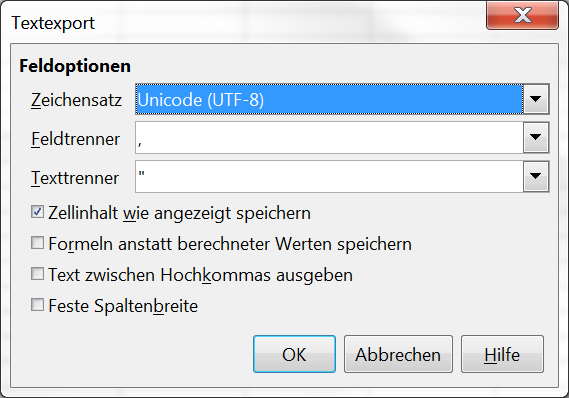
\includegraphics[width=0.6\textwidth]{bilder/tabelle_calcCSV}
\end{center}
  \caption{Der Dialog "`Textexport"' in LibreOffice Calc zur Speicherung von CSV-Dateien.}
\label{abb:tabelle-calcCSV}
\end{wrapfigure}
Mit der Option "`Zellinhalt wie angezeigt speichern"' wird der Inhalt der Zellen in der CSV-Datei so gespeichert, wie sie zu sehen sind. Wird die Option nicht ausgewählt, werden beispielsweise die Währungssymbole, die mittels Angaben für die Zellformatierung automatisch eingefügt wurden, nicht gespeichert. Die Option "`Formeln anstatt berechneter Werten speichern"' ermöglicht die Speicherung der eingegebenen Formeln anstatt der Werte.

TSV-Dateien werden in LibreOffice Calc oder OpenOffice Calc zunächst als CSV-Datei angelegt, wobei als Feldtrenner \{Tabulator\} gewählt wird. Um zu verdeutlichen, dass es sich um eine TSV-Datei und nicht um eine CSV-Datei handelt, sollte die Dateiendung nachträglich manuell geändert werden.

\subparagraph{Grafiken exportieren}
Grafiken, die in Tabellenkalkulationsprogrammen mittels der eingetragenen Daten erzeugt wurden, müssen für die Archivierung der Tabelle zusätzlich als gesonderte Bilddatei in einem geeigneten Format gespeichert werden. Passende Formate sind in den Kapiteln "`Rastergrafiken"' ab Seite \pageref{rastergrafiken} und "`Vektorgrafiken"' ab Seite \pageref{vektorgrafiken} beschrieben.

Der Export von Grafiken funktioniert bei LibreOffice Calc mit einem Klick mit der rechten Maustaste auf die Grafik. In dem erscheinenden Menü gibt es den Eintrag "`Als Bild exportieren"'. Es erscheint ein Speicherdialog für die Grafik in dem verschiedene Formate zur Auswahl stehen. Wird die Grafik als Rastergrafik gespeichert, muss vorher auf eine geeignete Größe der Grafik geachtet werden, indem sie beispielsweise vorher in der Tabellenkalkulation vergrößert wird.

Eine alternative Exportmethode, die auch in OpenOffice Calc und Microsoft Excel funktioniert, ist das Zwischenspeichern der Grafik und anschließende Speichern in einem dezidierten Grafikprogramm. Die Grafik kann in dem Grafikprogramm bearbeitet und angepasst werden, bevor sie gespeichert wird. Auch hier muss beim Speichern auf eine geeignete Größe des Bildes geachtet werden. 

Die oben beschriebenen Schritte müssen für alle Grafiken in der Tabellenkalkulation wiederholt werden, was bei Tabellenkalkulationen mit vielen Grafiken ein langwieriger Vorgang sein kann. Für diesen Fall bietet sich die Option an, die gesamte Tabellenkalkulation mittels "`Datei > Speichern unter"' als HTML-Datei ("`Webseite"' oder "`HTML-Dokument"') in einem gesonderten Ordner zu speichern. In dem Ordner werden alle Grafiken als PNG- oder JPG-Datei abgelegt. Bei dieser Exportvariante ist zu beachten, dass die erzeugten Einzelbilder eventuell Mängel in der Qualität aufweisen.


\subparagraph{Bereinigung von Tabellen}
Bei Tabellen, die über einen längeren Zeitraum von mehreren Bearbeitern gepflegt werden, können trotz festgelegter Vorgaben Inkonsistenzen auftreten. Solche Inkonsistenzen können beispielsweise darin bestehen, dass für die Materialbeschreibung mal "`Silber"' und mal "`Ag"' verwendet wird. Bei einer automatisierten statistischen Auswertung könnte das zu Verzerrungen führen. Für solche Fälle kann das frei verfügbare Programm OpenRefine verwendet werden. Es ermöglicht die Aufdeckung und Bereinigung von Inkonsistenzen in Tabellen. Darüber hinaus bietet es Funktionen, um die Daten zusätzlich über Transformationen oder durch externe Webinhalte anzureichern.

\begin{flushleft}
	OpenRefine: \urllist{http://openrefine.org/}
\end{flushleft}


\paragraph{Quellen}
\begin{flushleft}
Archaeology Data Service, Databases and Spreadsheets: A Guide to Good Practice \urllist{http://guides.archaeologydataservice.ac.uk/g2gp/DbSht_Toc}

T. Hicks, Should We Be Using ISO 12083?, The Journal of Electronic Publishing 3, 1998, 4 \urllist{http://quod.lib.umich.edu/j/jep/3336451.0003.407?view=text;rgn=main}

Research Data Management Service Group, Preparing tabular data for description and archiving \urllist{http://data.research.cornell.edu/content/tabular-data} 

\quelltyp{Formatspezifikationen}
ODT: \urllist{https://www.oasis-open.org/standards\#opendocumentv1.2}
XSLX: ECMA-376 \urllist{http://www.ecma-international.org/publications/standards/Ecma-376.htm}
CSV: RFC 4180 \urllist{https://tools.ietf.org/html/rfc4180}
TSV: IANA: \urllist{http://www.iana.org/assignments/media-types/text/tab-separated-values}
XML: OASIS (Hrsg.) Standards/Specs: Table Models \urllist{https://www.oasis-open.org/specs/tablemodels.php}
XML: OASIS (Hrsg.) XML Exchange Table Model Document Type Definition \urllist{https://www.oasis-open.org/specs/tm9901.html}
XML: TEI (Hrsg.) P5: Guidelines for Electronic Text Encoding and Interchange \urllist{http://www.tei-c.org/release/doc/tei-p5-doc/en/html/FT.html}
HTML: W3C: \urllist{http://www.w3.org/TR/html401/struct/tables.html}
ISO 12083: \urllist{http://www.iso.org/iso/catalogue_detail.htm?csnumber=20866}
TeX: \urllist{https://en.wikibooks.org/wiki/LaTeX/Tables}

\quelltyp{Tools und Programme}
OpenOffice Calc: \urllist{https://www.openoffice.org/}
LibreOffice Calc: \urllist{http://www.libreoffice.org/}
OpenRefine: \urllist{http://openrefine.org/}

\end{flushleft}